In diesem Kapitel werden die Implementierungen dieser Arbeit erläutert. Zuerst wird der Systemaufbau erklärt und alle verwendeten Module ausführlich beschrieben. Anschließend wird auf die verwendete Hardware eingegangen. Im Folgenden werden die implementierten Methoden des GA und der Zufallssuche genauer betrachtet, indem die exakten Methoden und künstlichen neuronalen Netze erklärt werden. Zum Schluss wird auf die implementierten Evaluationen und Auswertungen eingegangen. 

\section{Systemaufbau}
Das Gesamtsystem wird mit Python als Programmiersprache umgesetzt. Für die Implementierung werden zusätzliche Python Pakete verwendet. 
Für das Erstellen und Trainieren der künstlichen neuronalen Netze wird auf Tensorflow zurückgegriffen. Tensorflow ist eine End-to-End-Open-Source Plattform für maschinelles Lernen (ML). Zudem bietet Tensorflow ein umfassendes und flexibles Ökosystem aus Werkzeugen und Bibliotheken für ML-Anwendungen. Darüber hinaus hat Tensorflow eine starke Community, welche vorallem im ML-Bereich viele Open-Source-Projekte entwickelt und veröffentlicht.
Für die Zufallssuche wird SkLearn verwendet. Bei SkLearn handelt es sich um ein simples und effizientes Werkzeug zur prädiktiven Datenanalyse. Dies beinhaltet Funktionen wie:  Klassifikation, Regression, Clustering, Support Vektor Maschine. Mit Hilfe von SkLearn werden die bewertungsmatrixen zum Auswerten der Algorithmen umgesetzt.
Zum Darstellen von Diagrammen wird Seaborn und Matplotlib verwendet.
Der Genetische Algorithmus wurde eigenständig implementiert. Für diesen wurden nur die Pakete Numpy und Pandas verwendet. Numpy ist ein Paket für Multi-Dimensionen Arrays und bietet eine große Anzahl an mathematischen Funktionen. Pandas ist wie Numpy für Arrays und Datenframes zuständig. Im Detail ist Pandas für Datenstrukturen und Manipulation solcher Datenarrays entwickelt worden.
Da die Rechenzeit ein entscheidender Faktor der Optimierung darstellt, wird das Paket Multiprocessing verwendet. Dies führt vor allem bei Multi-Core-Servern zu schnelleren Berechnungen. Das Gesamtsystem wurde für CPU entwickelt. Darüber hinaus ist der Genetischen Algorithmus als GPU (engl. graphics processing unit) optimierte Implementierung vorhanden. Dies beschleunigt die Berechnungen von großen KNNs deutlich. 
All diese Einstellungen können per Argumente an das Python Skript übergeben werden. Somit ist es einfach möglich andere Berechnungen durchzuführen, auch solche, die in dieser Arbeit nicht besprochen werden. Eine ausführliche Auflistung aller verwendeten Pakete ist in Abbildung \ref{fig:Python_pakete} zu sehen. 

\begin{figure}[H]
  \centering  
  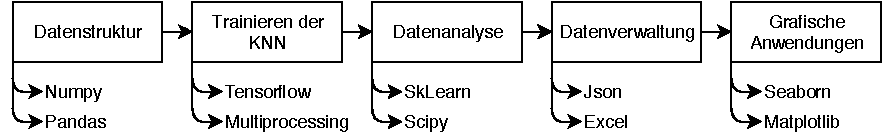
\includegraphics[scale=1]{img/Python_pakete.pdf}
  \caption{Datenfluss und verwendete Python Pakete, die zur Umsetzung der Arbeit verwendet wurden}
  \label{fig:Python_pakete}
\end{figure}

\subsection{Hardware}
Um die Optimierungen durchzuführen stehen drei Hardwaremöglichkeiten zur Auswahl. Dazu gehört ein Server mit i5-5550 Prozessoren mit 40 Kernen ohne GPU, ein Server mit einer Grafikkarte (Gtx1080Ti) um die Berechnungen durchzuführen und eine Server mit einem i7-7700 Prozessor mit 8 Kernen ohne GPU. Diese sind tabellarisch in Tabelle \ref{tab:Server} aufgeführt. Im späteren Kapitel \ref{sec:Evaluierung} wird auf die Benchmarks der Hardware eingegangen.

\begin{table}[htb]
\centering
\caption{Zur Verfügung stehende Hardware} \label{tab:Server}
\begin{tabular}{lccc}\toprule
\textbf{Hardwarekomponenten}	&\textbf{Server 1} &\textbf{Server 2} &\textbf{Server 3}	\\\midrule
Prozessor		& E5-2630   & i7-7700	& i7-7700 \\
Logische Kerne 	& 40        & 8     	& 8 	\\
Arbeitsspeicher	& 256 GB    & 8 GB	    & 32 GB	\\
Grafikkarte		& -	        & -	        & GTX 1080 Ti (11 GB)	\\\bottomrule
\end{tabular}
\end{table}


\subsection{Datensatz}
Um die künstlichen neuronalen Netze zu trainieren wurden Bilddaten als Daten-Grundlage ausgewählt. Bei den verwendeten Datensätzen handelt es sich um gängige Datensätze, die oft zum Vergleichen von Klassifikationsergebnissen von KNN genutzt werden. Folgende Datensätze wurden ausgewählt: Mnist Faschion, Mnist Digits und Cifar10. Diese drei Datensätze werden benutzt, da sie sich sehr ähnlich sind. Alle drei besitzen eine gleichmäßige Verteilung der Daten in Bezug auf die Klassen. Die Datensätze besitzen jeweils 10 Klassen. Die Besonderheit der Datensätze liegt auf ihrer guten Vergleichbarkeit. Die einzigen Unterschiede sind die Klassen und Bildformate. Alle verwendeten Datensätze werden wie folgt aufgeteilt: 65\% Trainingsdaten, 20\% Validierungsdaten, 15\% Testdaten. Somit wird das Overfitten der Netze verhindert, da die Daten klar getrennt werden. Nachfolgend werden die Datensätze genauer beschrieben.

\paragraph{Mnist Fashion Datensatz}
Zur Evaluierung der Methoden des Genetischen Algorithmus wurde der "`Mnist Fashion"' Datensatz benutzt. Dieser Datensatz enthält 10 Klassen für verschieden Kleidungsstücke. Er beinhaltet die Klassen: T-shirt/Top, Trouser, Pullover, Dress, Coat, Sandal, Shirt, Sneaker, Bag, Ankle Boot. Der Mnist Fashion Datensatz besteht aus 70.000 Schwarz-weiß Bildern mit je 28x28 Pixeln. Ein Beispiel aus dem Datensatz ist in Abbildung \ref{fig:dataset_example} auf der linken Seite zusehen. 

\paragraph{Mnist Digits Datensatz}
Zum Evaluieren der Optimierung des Fully Conneceted Netzes wird der "`Mnist Digits"' Datensatz benutzt. Dieser besteht aus handgeschrieben Ziffern zwischen 0 und 9. Der Mnist Digits Datensatz besteht aus 70.000 Schwarz-weiß Bildern mit je 28x28  Pixeln. Ein Beispiel des Mnist Digits Datensatze ist in der Mitte der Abbildung \ref{fig:dataset_example} zusehen. Um die Evaluation der Optimierung nicht nur mit einem Datensatz durchzuführen, wird ein dritter Datensatz verwendet.

\paragraph{Cifar 10 Datensatz}
Hierbei handelt es sich um den CIFAR 10 Datensatz. Er besitzt die Klassen: Flugzeug, Auto, Vogel, Katze, Reh, Hund, Pferd, Schiff und LKW. Der Datensatz ist aus 60.000 farbigen Bildern (RGB) mit je 32x32 Pixel aufgebaut. Ein Beispiel ist auf der rechten Seite der Abbildung \ref{fig:dataset_example} zusehen. 

\begin{figure}[H]
  \centering  
  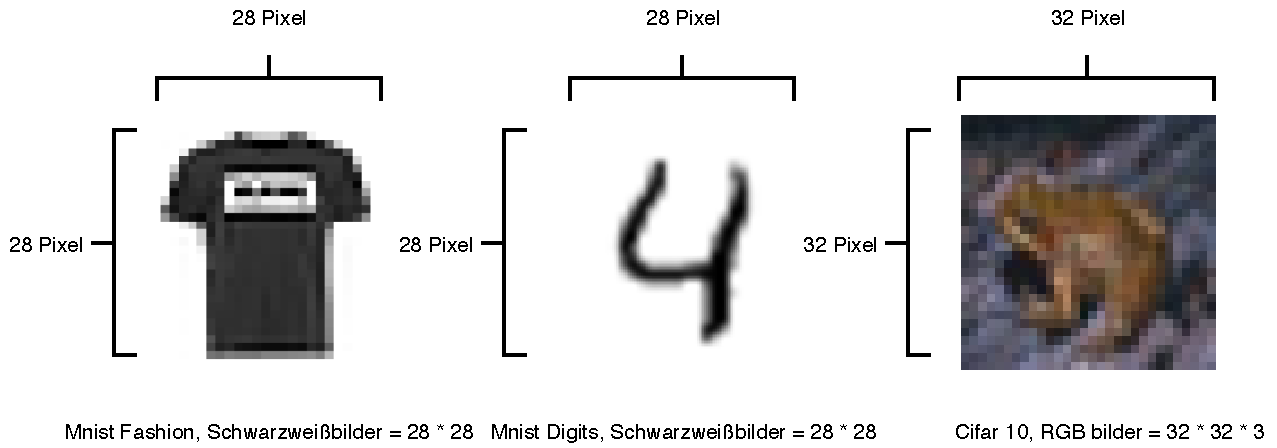
\includegraphics[scale=0.7]{img/dataset_example.pdf}
  \caption{Beispiele aus den verwendeten Datensätze}
  \label{fig:dataset_example}
\end{figure}

\section{Genetischer Algorithmus} \label{ssec:implementierung}
Die Implementierung des Genetischen Algorithmus entspricht den 5 Schritten des Genetischen Algorithmus, das Konzept wurde in Kapitel \ref{ssec:GA} beschrieben. In den folgenden Unterkapitel werden die implementierten Methoden im Detail besprochen. Zusätzlich wird auf speziellen Umsetzungen und Eigenschaften eingegangen. Da es zu den meisten Methoden in der Literatur wenig Informationen zu ihren Auswirkungen auf das Endergebnis gibt, wird ein Experiment zur Bestimmung der zielführenden Methoden durchgeführt. Für dieses Experiment wurde eine Optimierung der Hyperparameter durchgeführt. Als Netz wird ein Fully-Connected Netz mit einem Layer und 128 Neuronen verwendet, die Größe des Netzes wird im Abschnitt \ref{tab:fully_small} ausführlich beschrieben. Es wurde diese Größe gewählt, da die spätere Evaluation mit der gleichen Größe an Netz durchgeführt wird. Als Datengrundlage wurde der Mnist Fashion Datensatz verwendet, linke Seite der Abbildung \ref{fig:dataset_example}. Die Methoden mit den die besten Ergebnisse gefunden wurden, werden zur Evaluierung des Genetischen Algorithmus eingesetzt. Das Wissen zu den Grundlagen der Methoden des Genetischen Algorithmus wird für dieses Kapitel als voraussetzt angenommen und kann im Grundlagenkapitel \ref{Genetische_Algorithmen} nachgelesen werden.

\newpage

\subsection{Initialisierung der Anfangspopulation} \label{implementierung_init}
Die Größe der Anfangspopulation kann beliebig bestimmt werden. Im späteren Evaluationsabschnitt \ref{sec:Evaluierung} wird die genauen Größe definiert, da diese im direkten Zusammenhang mit der Laufzeit steht. Der Suchraum in dem die Hyperparameter zufällig initialisiert werden, ist in Tabelle \ref{tab:Rahmen} zusehen. Die Grenzen des Suchraums wurde mithilfe der Literatur und des beschriebenen Experiments bestimmt. Die Initialisierung im Suchraum ist zufällig mit einer gleichmäßigen Verteilung umgesetzt. Diese ist als Formel in Eq. \ref{eq:10} abgebildet.

\begin{equation}
	p(x) = \frac{1}{b - a}  \label{eq:10}
\end{equation}
a und b bilden die Intervallgrenzen.

\begin{table}[htb]
\centering
\caption{Suchraum des Genetischen Algorithmus}\label{tab:Rahmen}
\begin{tabular}{lccc}\toprule
\textbf{Hyperparameter}	&\textbf{Minimum}   &\textbf{Maximum}	\\\midrule
Prozessor		        & 0.000005          & 0.1 \\
Logische Kerne 	        & 0.05          	& 0.5 \\
Arbeitsspeicher     	& 10                & 80	\\
Grafikkarte		        & 0	                & 7	\\\bottomrule
\end{tabular}
\end{table}
Hierbei steht jede ganze Zahl beim Optimierer für einen eigenen Optimierer. Hierbei entspricht: 0 = adam, 1 = SGD, 2 = RMSprop, 3 = Adagrad, 4 = adadelta, 5 = adammax, 6 = nadam, 7 = ftrl


\subsection{Fitnessfunktion}\label{implementierung_Fitnessfunktion}
Die Fitnessfunktion beinhaltet den rechenaufwendigsten Teil der Arbeit. In dieser werden die KNNs berechnet. Dazu werden die Gene (Hyperparameter) als Input verwendet. Anschließend werden die Daten geladen, das Netz trainiert und anschließend evaluiert. Der Rückgabewert ist die Klassifizierungsgenauigkeit, die dem Fitnesswert entspricht. Die Fitnessfunktion ist in Abbildung \ref{fig:Fitnessfunktion} als Whitebox dargestellt. Die Fintessfunktion wird für unterschiedliche KNN erstellt. Diese Netze sind im Kapitel \ref{sec:Evaluierung} beschreiben.

\noindent%
\begin{figure}[H]
  \centering  
  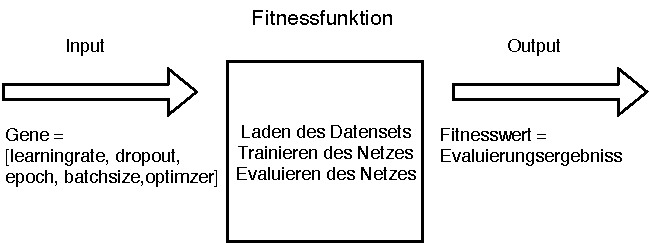
\includegraphics[scale=1]{img/Fitnessfunction.pdf}
  \caption{Beispielhafte Whitebox der Fitnessfunktion mit Genen als Input und Klassifikationsgenauigkeit als Output}
  \label{fig:Fitnessfunktion}
\end{figure}  


\subsection{Selektion der Eltern} \label{implementierung_Selektion_Eltern}
Aus dem Experiment hat sich gezeigt, dass bei der Selektion der Eltern die Fitness proportional Selektion(FPS) die besseren Ergebnisse im Vergleich zu der Ranking Selektion liefert. Aus diesem Grund wird die FPS bei der Evaluation des Genetischen Algorithmus verwendet.

\subsubsection{Vermehrung} \label{implementierung_vermehrung}
Für das \textbf{Crossover} wurde Two-Point Crossover und Uniform-Crossover implementiert. Für die \textbf{Mutation} wurde die Gauss-Mutation mit der Gaussdichteverteilung, mit Sigma gleich 0.1 (Eq. \ref{eq:11}) und eine Mutation mit gleichmäßiger Verteilung (Eq. \ref{eq:10}) implementiert. Für die spätere Evaluation der Optimierung mit dem GA wurde Two-Point Crossover und die Gauss-Mutation ausgewählt, da sie in den Experimenten die zielführendsten Ergebnisse lieferten.

\begin{equation}
	p(x) = \frac{1}{\sqrt{ 2 \pi \sigma^2 }} e^{ - \frac{ (x - \mu)^2 } {2 \sigma^2} } \label{eq:11}
\end{equation} 

\newpage

\subsection{Neue Generation}
Die Population der neuen Generation wird mit den genannten Methoden ausgewählt. Diese sind in Abbildung \ref{fig:Ga_Methoden} noch einmal dargestellt. Die Experimente zeigten, dass die Optimierungsergebnisse sich steigern lassen, wenn die besten zwei Individuen der alten Generation, ohne Mutation und Crossover, in die nächste Generation übergeben werden. Dies kann für beliebig viele Generationen durchgeführt werden oder bis zum Erreichen einer Abbruchbedingung.

\noindent%
\begin{figure}[H]
  \centering  
  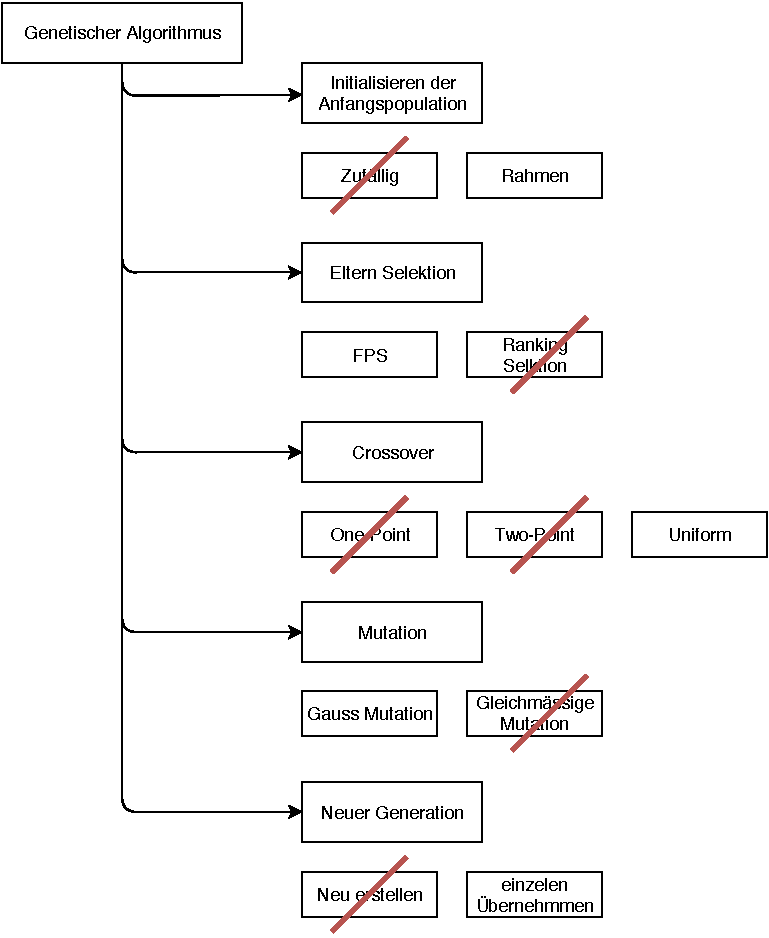
\includegraphics[scale=0.9]{img/Ga_Methoden.pdf}
  \caption{Implementierte und verwendete Methoden des Genetischen Algorithmus}
  \label{fig:Ga_Methoden}
\end{figure}

\section{Zufallssuche}
Die Zufallssuche wird mit Hilfe der Python Bibliothek SkLearn umgesetzt. Die implementierte Zufallssuche ist, wie im Grundlagenkapitel \ref{Zufalls_Suche} beschrieben, aufgebaut. Für den Suchraum der Zufallssuche gelten die gleichen Rahmenbedingungen wie für den Genetischen Algorithmus. Im Vergleich zum GA wird der Suchraum bei der Zufallssuche in ein Raster aufgeteilt. Dieses Raster ist in Tabelle \ref{tab:Raster} zusehen.


\begin{table}[htb]
\caption{Suchraum der Zufallssuche} \label{tab:Raster}
\begin{tabular}{lccclllll}\toprule
\textbf{Hyperparameter} &\textbf{Min}   &   &   &   &   &  &   &\textbf{Max}	\\\midrule
Lernrate       & 0.00005 & 0.0001 & 0.0005 & 0.001 & 0.005 & 0.01 & 0.05 & 0.1  \\
Dropout        & 0.05    & 0.1    & 0.2    & 0.3   & 0.4   & 0.5  & 0.6  & 0.7  \\
Epochen        & 10      & 20     & 30     & 40    & 50    & 60   & 70   & 80   \\
Batchsize      & 8       & 16     & 32     & 40    & 48    & 56   & 64   & 72   \\
Optimizer      & 0       & 1      & 2      & 3     & 4     & 5    & 6    & 7    \\\bottomrule
\end{tabular}
\end{table}

Jede ganze Zahl des Optimizer steht für einen eigenen Optimierer. Hierbei entspricht 0 = adam, 1 = SGD, 2 = RMSprop, 3 = Adagrad, 4 = adadelta, 5 = adammax, 6 = nadam, 7 = ftrl.

\section{Evaluierung} 
\label{sec:Evaluierung}
Zur Evaluierung wird die Berechnungszeit der beiden Algorithmen gleichgesetzt. Da das Trainieren der KNN 95\% der Berechnungszeit der Algorithmen ausmacht, wird die Berechnungszeit über die Anzahl der Trainingsvorgänge begrenzt. Durch Versuche ergab sich die Evaluierung von 50 und 250 Iterationen als zielführend. Eine weitere Verdopplung der Iterationen von 250 auf 500, zeigte bei den Versuchen keine Verbesserung der Ergebnisse. Trotz des doppelten Rechenaufwandes. Aus diesem Grund ist die Berechnung von 500 Iterationen nicht umgesetzt worden. Für die Zufallssuche ergibt sich somit 50 und 250 Iterationen. Für den Genetischen Algorithmus ergibt sich für 50 Iterationen eine Populationsgröße von 25 Individuen mit 2 Generationen. Für 250 Iterationen wird im GA eine Populationsgröße von 50 Individuen und 5 Generationen gewählt. Um aussagekräftige Ergebnisse zu erhalten wurden zwei KNNs implementiert:


\subsection{Hyperparameter Optimierung - Fully Connected Network}
Es wird ein Fully Connected Network zur Klassifizierung von handgeschriebenen Ziffern implementiert. Darüber hinaus werden zwei verschiedene Größen des künstlichen neuronalen Netzes implementiert, um mögliche Unterschiede der Modellgröße auf die Optimierung zu erkennen. Für das Fully-Connected-Network wurden diese Größen von KNNs implementiert:
\begin{itemize}
\item \textbf{kleines KNN} mit einem Layer und 128 Neuronen. Die exakte Modell-Architektur ist in der nachfolgenden Auflistung zusehen. Die 28x28 Pixel der Eingangsdaten werden zu 784 Pixel mit nur einer Dimension flachgedrückt (engl. flatted). Anschließend kommt die Versteckteschicht (engl. hidden Layer) mit 128 Neuronen und einer  Dropoutschicht, die für jedes Neuron durchgeführt wird. Abschließend kommt die Ausgangsschicht mit 10 Klassen, wodurch sich 10 Neuronen in der Ausgangsschicht ergeben. Dies entspricht einer Anzahl von 101.770 trainierbaren Parametern. Somit ist dieses Netz im Vergleich zu State-of-the-Art Netzen relativ klein. Diese Netz ist beispielhaft als Figur \ref{fig:mlp_128} und als Auflistung in der Liste \ref{auflistung_fully_klein} zusehen.

\noindent%
\begin{figure}[H]
  \centering  
  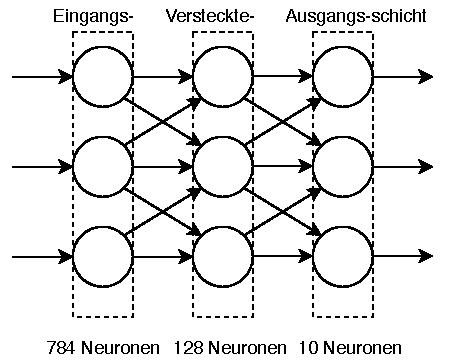
\includegraphics[scale=0.9]{img/mlp_128.pdf}
  \caption{Beispielhafte Darstellung des kleinen KNNs}
  \label{fig:mlp_128}
\end{figure}


Beispielhaft wird die Trainingsdauer des kleinen Netzes für 10 und 80 Epochen evaluiert. Bei 10 Epochen dauerte der Trainingsvorgang 34 Sekunden und für 80 Epochen 252 Sekunden. Diese Werte wurden auf einem Intel i7-7700 3,6 GHz erreicht.
\newpage
{\small
\begin{lstlisting}[language=C,caption=Exakte Modell-Architektur des kleinen Fully-Conneted-Networks,label=auflistung_fully_klein]
_______________________________________________________________
Layer (type)                 Output Shape              Param #
===============================================================
flatten (Flatten)            (None, 784)               0
_______________________________________________________________
dense (Dense)                (None, 128)               100480
_______________________________________________________________
dropout (Dropout)            (None, 128)               0
_______________________________________________________________
dense_1 (Dense)              (None, 10)                1290
===============================================================
Total params: 101,770
_______________________________________________________________
\end{lstlisting}
}

\item \textbf{großes KNN} mit zwei Layer je 128 Neuronen. Die exakte Modell-Architektur ist in der nachfolgenden Auflistung zusehen. Die 28x28 Pixel der Inputdaten werden zu 784 Pixel mit nur einer Dimension flachgedrückt. Anschließend kommt die erste Versteckteschicht mit 128 Neuronen und einer Dropoutschicht, die für jedes Neuron durchgeführt wird. Nun kommt erneut eine Versteckteschicht und Dropout mit 128 Neuronen. Abschließend kommt die Ausgangsschicht mit 10 Klassen, wodurch sich 10 Neuronen in der Ausgangsschicht ergeben. Dies entspricht einer Anzahl von 134.794 trainierbaren Parametern. Somit ist das Netz im Vergleich zu State-of-the-Art Netzen relativ klein. Diese Netz ist beispielhaft als Figur \ref{fig:mlp_2x128} und als Auflistung in der Liste \ref{auflistung_fully_groß} zusehen.

\noindent%
\begin{figure}[H]
  \centering  
  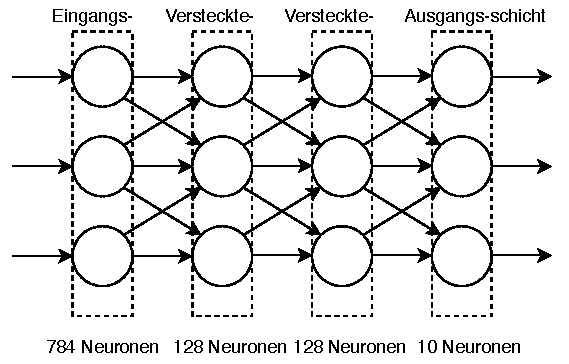
\includegraphics[scale=0.9]{img/mlp_2x128.pdf}
  \caption{Beispielhafte Darstellung des großen KNNs}
  \label{fig:mlp_2x128}
\end{figure}

Beispielhaft wird die Trainingsdauer des großen Netzes für 10 Epochen und 80 Epochen evaluiert. Bei 10 Epochen dauerte der Trainingsvorgang 44 Sekunden und für 80 Epochen 339 Sekunden. Diese Werte wurden auf einem Intel i7-7700 3,6 GHz erreicht. 

{\small
\begin{lstlisting}[language=C,caption=Exakte Modell-Architektur des großen Fully-Conneted-Networks,label=auflistung_fully_groß]
_______________________________________________________________
Layer (type)                 Output Shape              Param #
===============================================================
flatten (Flatten)            (None, 784)               0
_______________________________________________________________
dense (Dense)                (None, 128)               100480
_______________________________________________________________
dropout (Dropout)            (None, 128)               0
_______________________________________________________________
dense_1 (Dense)              (None, 128)               16512
_______________________________________________________________
dropout_1 (Dropout)          (None, 128)               0
_______________________________________________________________
dense_2 (Dense)              (None, 128)               16512
_______________________________________________________________
dropout_2 (Dropout)          (None, 128)               0
_______________________________________________________________
dense_3 (Dense)              (None, 10)                1290
===============================================================
Total params: 134,794
_______________________________________________________________
\end{lstlisting}
}


\end{itemize}

\subsection{Hyperparameter Optimierung - Convolutional Neural Network}
Es wurde ein faltendes neuronales Netz (engl. Convolutional Neural Network - CNN) zur Klassifizierung von kleinen RGB Bildern aus dem Cifar10 Datensatz implementiert. Die exakte Modell-Architekturen ist in der nachfolgenden Auflistung zusehen.
Beim CNN werden die Pixel nicht flachgedrückt, sondern können als Matrix geladen werden. Anschließend kommen verschiedene Kombinationen aus Convolutionalschicht, Activationschicht, Dropoutschicht und Maxpoolingschicht. Diese Schichten besitzen deutlich mehr Parameter. Dieses CNN besitzt 1.250.858 trainierbare Parameter und besitzt damit fast 10 Fach so viele trainierbaren Parametern wie die FCN.

Beispielhaft wird die Trainingsdauer des CNN-Netzes für 10 und 80 Epochen evaluiert. Bei 10 Epochen dauerte der Trainingsvorgang 15 Minuten und für 80 Epochen 125 Minuten. Diese Werte wurden auf einem Intel i7-7700 3,6 GHz erreicht. 

{\small
\begin{lstlisting}[language=C,caption=Exakte Modell-Architektur des Convolutional Neural Network ,label=auflistung_cnn]
_______________________________________________________________
Layer (type)                 Output Shape              Param #
===============================================================
conv2d (Conv2D)              (None, 32, 32, 32)        896
_______________________________________________________________
activation (Activation)      (None, 32, 32, 32)        0
_______________________________________________________________
conv2d_1 (Conv2D)            (None, 30, 30, 32)        9248
_______________________________________________________________
activation_1 (Activation)    (None, 30, 30, 32)        0
_______________________________________________________________
max_pooling2d (MaxPooling2D) (None, 15, 15, 32)        0
_______________________________________________________________
dropout_1 (Dropout)          (None, 15, 15, 32)        0
_______________________________________________________________
conv2d_2 (Conv2D)            (None, 15, 15, 64)        18496
_______________________________________________________________
activation_2 (Activation)    (None, 15, 15, 64)        0
_______________________________________________________________
conv2d_3 (Conv2D)            (None, 13, 13, 64)        36928
_______________________________________________________________
activation_3 (Activation)    (None, 13, 13, 64)        0
_______________________________________________________________
max_pooling2d_1 (MaxPooling2 (None, 6, 6, 64)          0
_______________________________________________________________
dropout_2 (Dropout)          (None, 6, 6, 64)          0
_______________________________________________________________
flatten_1 (Flatten)          (None, 2304)              0
_______________________________________________________________
dense_2 (Dense)              (None, 512)               1180160
_______________________________________________________________
activation_4 (Activation)    (None, 512)               0
_______________________________________________________________
dropout_3 (Dropout)          (None, 512)               0
_______________________________________________________________
dense_3 (Dense)              (None, 10)                5130
_______________________________________________________________
activation_5 (Activation)    (None, 10)                0
===============================================================
Total params: 1,250,858
_______________________________________________________________
\end{lstlisting}
}

\subsection{Hyperparameter Optimierung - kleiner Datensatz}
Bei der Optimierung mit kleinen Datensätzen wird geprüft, ob sich andere Ergebnisse beim Optimieren der Hyperparameter mit kleinerem Datensatz zeigen. Dazu werden die gleichen Datensätze und Netze wie in den vorherigen Evaluierungen verwendet. Nur wird in diesem Fall, die Trainingsdatensätze um 90\% der vorhanden Daten verkleinert. Der Anteil an Testdaten bleibt gleich, so werden die Endergebnisse auf dem gleichen Daten evaluiert.

\subsection{Versuch der Modell-Architektur Optimierung}
Abschließend wird ein Versuch zur Optimierung der Modell-Architektur eines klassifizierungs Netzes implementiert. Für diese Optimierung wird ein Fully-Connected-Network verwendet. Zur Umsetzung der Modell-Architektur Optimierung werden die Neuronen pro Schicht als Gene umgesetzt, zusehen in Abbildung \ref{fig:gene_neuronen}. In diesem Versuch werden die Gene mit drei Schichten umgesetzt. Für die Neuronen pro Schicht, wird ein Minimum von 10 Neuronen und ein Maximum von 256 Neuronen, festgelegt. Mithilfe des Versuches soll eine optimale Modell-Architektur gefunden werden. Es werden die Hyperparameter des ersten Versuchs verwendet.

\begin{figure}[H]
  \centering  
  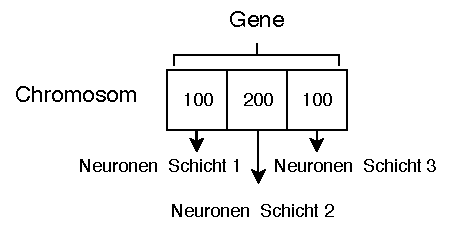
\includegraphics[scale=1.5]{img/gene_neuronen.pdf}
  \caption{Beispielhafte Zeichnung des Chromosom eines Individuums in welchem die Neuronen als Gene realisiert wurden}
  \label{fig:gene_neuronen}
\end{figure}

\subsection{Auswertung}
Alle Ergebnisse werden automatisch mit den dazugehörigen Konfigurationen und Berechnungen in einer Json-Datei abgespeichert. Aus dieser Json-Datei wird dann automatisch eine Zusammenfassung aller Ergebnisse erstellt und anschließend in einer Excel Datei abgespeichert. Des Weiteren werden Dichte Diagramme aus den Json-Dateien zu den einzelnen Hyperparametern automatisch erstellt und gespeichert. In diesen werden die Dichteverteilungen der einzelnen Hyperparameter in Bezug auf die Fitness dargestellt. Somit können die Hyperparameter intuitiv ausgewählt werden. Der Ablauf der Auswertung ist schematisch in Abbildung \ref{fig:implementierung_auswertung} abgebildet. 

\begin{figure}[H]
  \centering  
  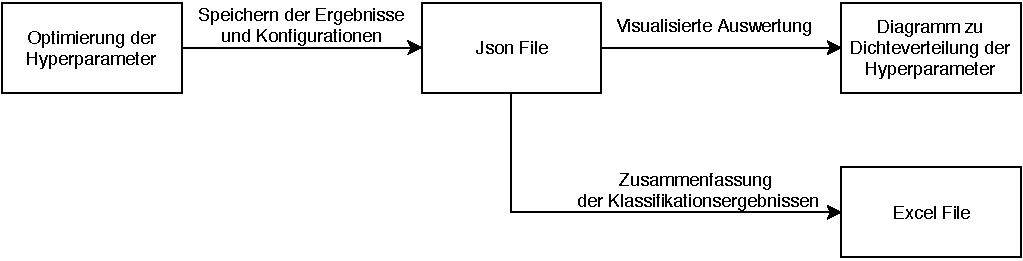
\includegraphics[scale=0.9]{img/Auswertung.pdf}
  \caption{Datenstruktur der Auswertung}
  \label{fig:implementierung_auswertung}
\end{figure}


\section{Zusammenfassung}
In diesem Kapitel wurde auf die implementierten Optimierungsalgorithmen und künstlichen neuronalen Netzen eingegangen. Dazu wurde zuerst der Systemaufbau, Programmiersprache und alle dazu gehörigen Python-Pakete und ihre jeweilige Funktion erläutert. Nachfolgend wurde auf die Hardware, die zur Verfügung stand, eingegangen. Danach wurden die verwendeten Datensätze: Mnist Fashion, Mnist Digits und der Cifar10 Datensatz erklärt. Bei allen drei handelt es sich um Bilddatensätze, welche mit 28x28 Pixel und 32x32x3 Pixel, relativ kleine Bilddaten enthalten. Anschließend wird erläutert, welche 5 Schritte für den Genetischen Algorithmus implementiert wurden, sowie die Methoden, die zur Evaluierung des GA eingesetzt werden. Ebenso wird die implementierte Zufallssuche erläutert welche zum Vergleich des GA dient. Beide Algorithmen benutzen die gleichen Datensätze, als auch die gleichen künstlichen neuronalen Netze. Als KNNs werden ein Fully Conneted Netz mit zwei Variationen optimiert und ein Convolutional Neuronal Network verwendet. Zum Abspeichern der Netze werden Json und Excel Files benutzt. Aus diesen Files werden dann die Auswertungen bzw. das Dichte-Diagramm bestimmt.